% !TeX program = xelatex
\documentclass[10pt,a4paper]{ctexart} % 设置文章类型，正文字号与纸张大小

% 页面与正文常用宏包
\usepackage[margin=2cm]{geometry} % 设置页面四周页边距
\usepackage{graphicx}             % 插入图片
\usepackage{amsmath}              % 提供cases、aligned等数学公式环境
\usepackage{amssymb}              % 提供\therefore等扩展数学符号
\usepackage{booktabs}             % 提供\toprule、\midrule、\bottomrule三线表命令
\usepackage{float}                % 提供[H]固定图片、表格位置
\usepackage{subcaption}           % 提供subfigure子图环境及子图标题
\usepackage{wrapfig}              % 提供wrapfigure图文环绕环境
\usepackage{fancyhdr}             % 自定义页眉和页脚
\usepackage{hyperref}             % 生成超链接

% 页眉页脚
\pagestyle{fancy}                  % 启用fancyhdr定义的页面样式
\fancyhf{}                         % 清空默认页眉和页脚
\fancyfoot[C]{\thepage}            % 在页脚中央显示页码
\renewcommand{\headrulewidth}{0pt} % 隐藏页眉横线
\renewcommand{\footrulewidth}{0pt} % 隐藏页脚横线

% 超链接
\hypersetup{
  colorlinks=true,                % 使用彩色文字链接，而非带边框的链接
  linkcolor=red,                 % 目录、公式及图表交叉引用的颜色
  filecolor=cyan,                 % 本地文件链接的颜色
  urlcolor=blue,                  % 网址链接的颜色
  pdftitle={交流电路功率因数实验预习报告},     % 写入PDF文档属性的标题
  bookmarksnumbered=true          % PDF书签显示章节编号
}

% 定义字号命令
\newcommand{\chuhao}{\fontsize{42pt}{63pt}\selectfont}
\newcommand{\xiaochu}{\fontsize{36pt}{54pt}\selectfont}
\newcommand{\yihao}{\fontsize{26pt}{39pt}\selectfont}
\newcommand{\xiaoyi}{\fontsize{24pt}{36pt}\selectfont}
\newcommand{\erhao}{\fontsize{22pt}{33pt}\selectfont}
\newcommand{\xiaoer}{\fontsize{18pt}{27pt}\selectfont}
\newcommand{\sanhao}{\fontsize{16pt}{24pt}\selectfont}
\newcommand{\xiaosan}{\fontsize{15pt}{22.5pt}\selectfont}
\newcommand{\sihao}{\fontsize{14pt}{21pt}\selectfont}
\newcommand{\xiaosi}{\fontsize{12pt}{18pt}\selectfont}
\newcommand{\wuhao}{\fontsize{10.5pt}{15.75pt}\selectfont}
\newcommand{\xiaowu}{\fontsize{9pt}{13.5pt}\selectfont}

% 章节格式
\ctexset{
  section={
    format={\CJKfontspec[AutoFakeBold=2.5]{KaiTi}\sanhao\bfseries}, % 一级标题使用三号加粗楷体
    name={,、},                                                    % 在中文章节序号后添加顿号
    number=\chinese{section},                                      % 一级标题编号使用“一、二、三”形式
    aftername={}                                                   % 取消编号与标题文字之间的空格
  },
  subsection={
    format={\CJKfontspec[AutoFakeBold=2.5]{KaiTi}\sihao\bfseries}, % 二级标题使用四号加粗楷体
  },
  subsubsection={
    format={\CJKfontspec[AutoFakeBold=2.5]{KaiTi}\xiaosi\bfseries}, % 三级标题使用小四加粗楷体
  }
}

\begin{document}

% 封面
\thispagestyle{fancy} % 封面保留底部居中的页码
\fancyfoot[C]{\thepage}
\begin{center}
  \CJKfontspec[AutoFakeBold=2.5]{KaiTi}\bfseries % 封面中文使用楷体并人工加粗，西文同时加粗
  \vspace*{2.0cm}
  \xiaochu 
    物理实验预习报告

  \vspace{3.8cm}
  \begin{minipage}{10.0cm}
    \sanhao
    \makebox[2.6cm][l]{实验名称：}
    \underline{\makebox[7.0cm][c]{交流电路功率因数实验}}\par\vspace{12pt}

    \makebox[2.6cm][l]{指导老师：}
    \underline{\makebox[7.0cm][c]{施博通}}\par\vspace{12pt}
  \end{minipage}

  \vspace{3.8cm}
  \begin{minipage}{10.0cm}
    \sihao
    \makebox[1.4cm][l]{班级：}
    \underline{\makebox[8.0cm][c]{}}\par\vspace{10pt}

    \makebox[1.4cm][l]{姓名：}
    \underline{\makebox[8.0cm][c]{IllusoryRain}}\par\vspace{10pt}

    \makebox[1.4cm][l]{学号：}
    \underline{\makebox[8.0cm][c]{}}
  \end{minipage}

  \vspace{1.8cm}
  \sihao
    实验日期：
    \underline{\makebox[0.7cm][c]{2026}}年
    \underline{\makebox[0.7cm][c]{9}}月
    \underline{\makebox[0.7cm][c]{23}}日
    星期\underline{\makebox[0.7cm][c]{三}}上午

  \vspace{0.7cm}
  \sihao 
    浙江大学物理实验教学中心
\end{center}

\newpage
\xiaosi\songti\mdseries % 后续正文统一使用小四不加粗的宋体

\section{预习报告（10分）}

  \subsection{实验综述（5分）}
  
    \subsubsection{实验背景}
    交流电功率因数：
     \[
    P=UI\cos\varphi
    \]

    提高交流电功率因数的意义：
    \begin{itemize}
      \item 提高用电利用率
      \item 减少输电线路的损耗
      \item 改善电压质量
      \item 降低用电成本
    \end{itemize}

    \begin{figure}[H]
      \centering
      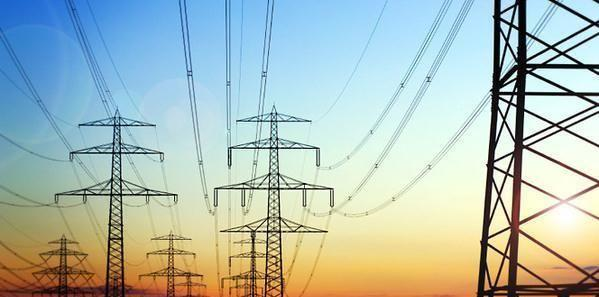
\includegraphics[width=0.6\textwidth]{figures/图1.png}
      \caption{生活中的交流电线}
    \end{figure}

    \subsubsection{交流电功率因数}
    \begin{wrapfigure}{r}{0.25\textwidth}
      \centering
      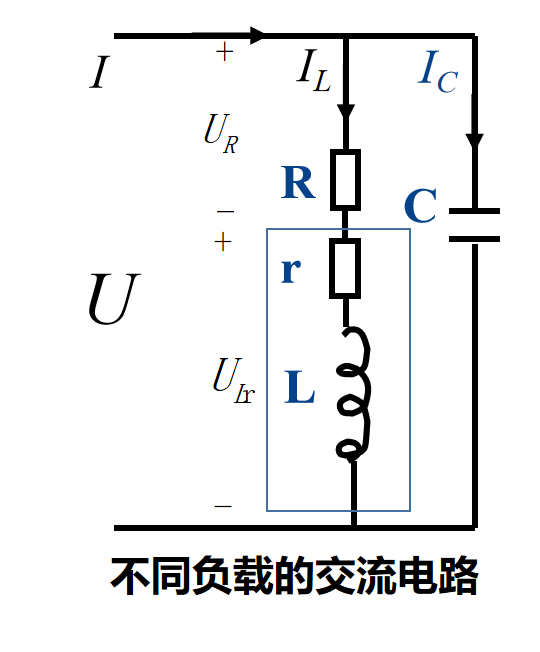
\includegraphics[width=\linewidth]{figures/图2.png}
      \caption{不同负载的交流电路}
    \end{wrapfigure}

    交流电路中的元件有阻性负载、容性负载、感性负载。
    \begin{itemize}
      \item 阻性负载：靠发热来工作的电器都是阻性负载, 阻性负载的特点是，电流和电压同步变化，相位差为“零度”，工作时会产生热量。
      \item 容性负载：电容上电流超前电压90°相位，设想一个电容与电阻串联充电。从充电过程看，总是先有流动电荷（即电流）的积累才有电容上的电压变化，即电流总是超前于电压。
      \item 感性负载：像我们平时用的日光灯等家用电器。电感上电流落后感应电压90°相位。
    \end{itemize}

    如果以电流$I_L$作为相位参考，图3为各物理量之间的相位矢量图。
    由图可见，$I_L$与$U_R$同相；纯电感$L$两端的电压$U_L$比$I_L$超前$\pi/2$。
    合成电压$U$的大小为总电压的幅值，$\varphi$为 $I_L$ 落后于$U$的相位角。

    对应提高电感性电路的功率因数，常用的方法就是在靠近感性负载端并联电容器，其电路图如图4所示，
    由相量图可知原感性负载电流滞后于电压$\varphi$，当并联电容以后，只要电容的大小选择得当，
    就可以使并联电容以后的总电流小于原来电感中的电流，使$\varphi'<\varphi$，使功率因数得到提高。 

    \begin{figure}[H]
      \centering
      \begin{minipage}{0.4\textwidth}
        \centering
        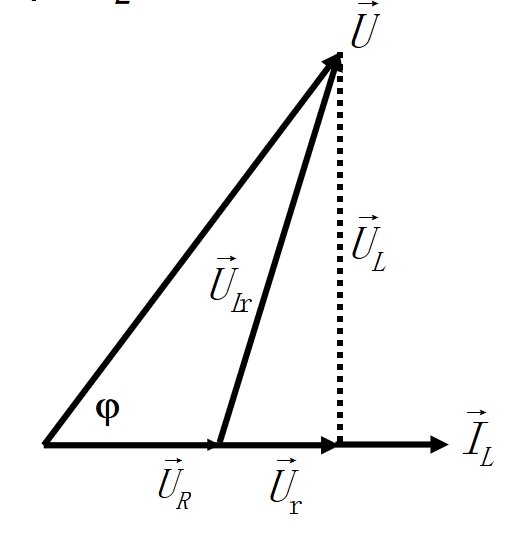
\includegraphics[width=\linewidth]{figures/图3.png}
        \caption{相位矢量图}
      \end{minipage}
      \hfill
      \begin{minipage}{0.4\textwidth}
        \centering
        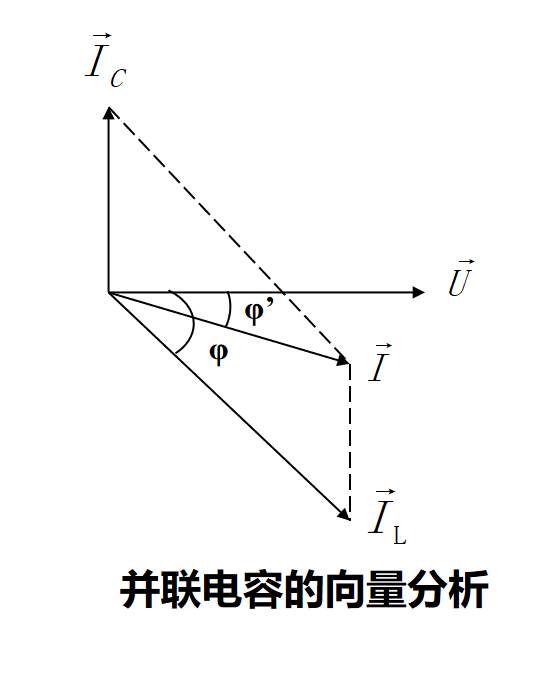
\includegraphics[width=\linewidth]{figures/图4.png}
        \caption{并联电容的向量分析}
      \end{minipage}
    \end{figure}

    \subsubsection{日光灯管的工作原理}
    日光灯电路是日常照明电路中一种较为经济的照明电路，也是一种典型的电感性负载电路，它主要由灯管、镇流器、启辉器组成。

    镇流器是一个带铁芯的自感线圈，自感系数很大。

    启辉器主要是一个充有氖气的小氖泡，里面装有两个电极，一个是静触片，一个是由两个膨胀系数不同的金属制成的U型动触片
    （双层金属片——当温度升高时，因两层金属片的膨胀系数不同，且内层膨胀系数比外层膨胀系数高，所以动触片在受热后会向外伸展）。

    \begin{figure}[H]
      \centering
      \begin{minipage}{0.35\textwidth}
        \centering
        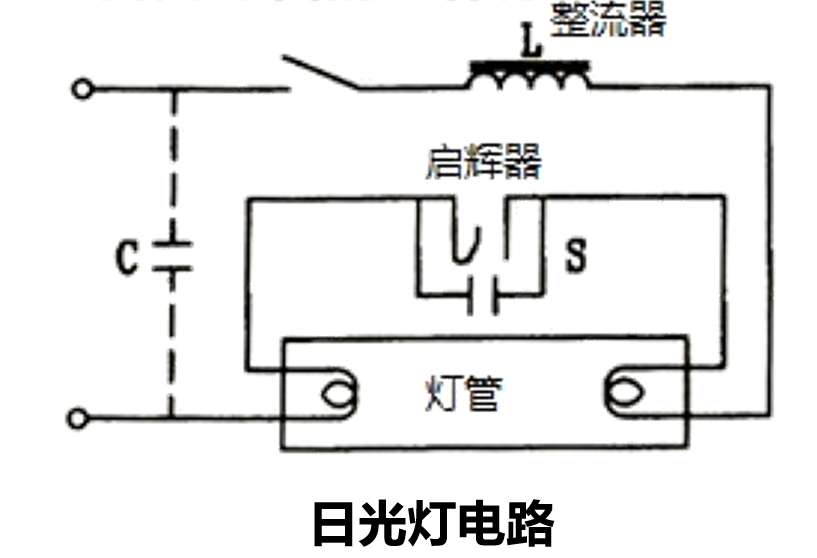
\includegraphics[width=\linewidth]{figures/图5.png}
        \caption{日光灯电路}
      \end{minipage}
      \hfill
      \begin{minipage}{0.35\textwidth}
        \centering
        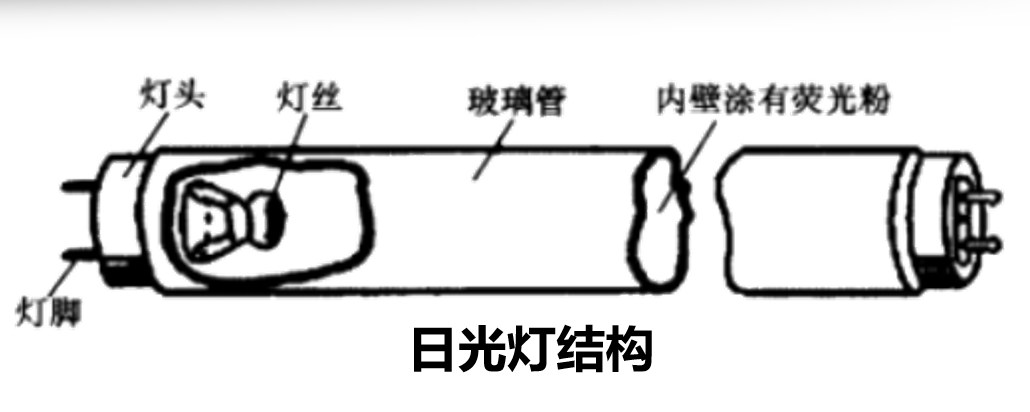
\includegraphics[width=\linewidth]{figures/图6.png}
        \caption{日光灯结构}
      \end{minipage}
      \hfill
      \begin{minipage}{0.15\textwidth}
        \centering
        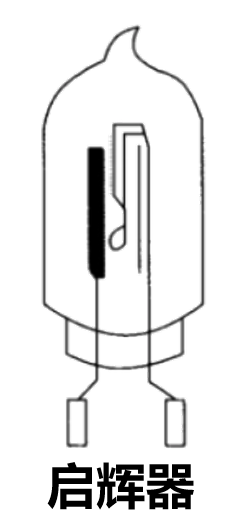
\includegraphics[width=\linewidth]{figures/图7.png}
        \caption{启辉器}
      \end{minipage}
    \end{figure}

  \subsection{实验重点（3分）}
  \begin{enumerate}
    \item 理解功率因数的物理意义；
    \item 掌握提高电感性电路功率因素的方法；
    \item 熟悉日光灯的工作原理，掌握测量日光灯功率的方法。
  \end{enumerate}

  \subsection{实验难点（2分）}
  \begin{enumerate}
    \item 理解并联电容器对交流电路功率因数的影响；
    \item 分析并联电容后电路电流的变化；
    \item 准确测量$U$、$I$和$P$，计算不同电容量下的功率因数并分析其变化规律。
  \end{enumerate}

\vspace*{\fill} % 使下面内容在页面底部显示
\noindent
\begin{minipage}{\textwidth}
  注意事项：

  \begingroup
    \setlength{\leftskip}{2em} % 1--4整体向右缩进两个汉字宽度
    1. 用PDF格式上传“实验报告”，文件名：学生姓名+学号+实验名称+周次。

    2. “实验报告”必须递交在“学在浙大”本课程内对应实验项目的“作业”模块内。

    3. “实验报告”成绩必须在“浙江大学物理实验教学中心网站”-“选课系统”内查询。

    4. 教学评价必须在“浙江大学物理实验教学中心网站”-“选课系统”内进行，学生必须进行教学评价，才能看到实验报告成绩，教学评价须在本次实验结束之后3天内进行。\par
  \endgroup

  \begin{center}
    {\CJKfontspec[AutoFakeBold=2.5]{SimSun}\bfseries 浙江大学物理实验教学中心制}
  \end{center}
\end{minipage}

\end{document}
